\chapter{Návrh}
\label{sec:de}

\section{Návrhový vzor MVC}
\label{sec:de_mvc}

Struktura nadřazeného systému je vhodná k~použití návrhového vzoru MVC, tedy \textit{model-view-controller}. \textit{Model} zde představují garáže (podřízené systémy), k~nim vázané události a logika jejich vyhodnocování. 

\textit{View} je zobrazení těchto dat, tedy především generované HTML stránky webového rozhraní. Jako další \textit{view} je možné považovat získávání dat (například ve formátu JSON) pomocí API nadřazeného systému, třeba při zasílání registračních klíčů podřízeným systémům.

\textit{Controller} je pak část aplikace, která se stará o~zpracování HTTP požadavků. Ty mohou přicházet jednak z~uživateloval prohlížeče, jednak od podřízených systémů. Na základě těchto požadavků pak \textit{controller} posílá příslušné příkazy \textit{modelu}. Struktura aplikace při použití vzoru MVC je naznačena na obrázku \ref{fig:mvc}.

\begin{figure}[h!]
    \centering
    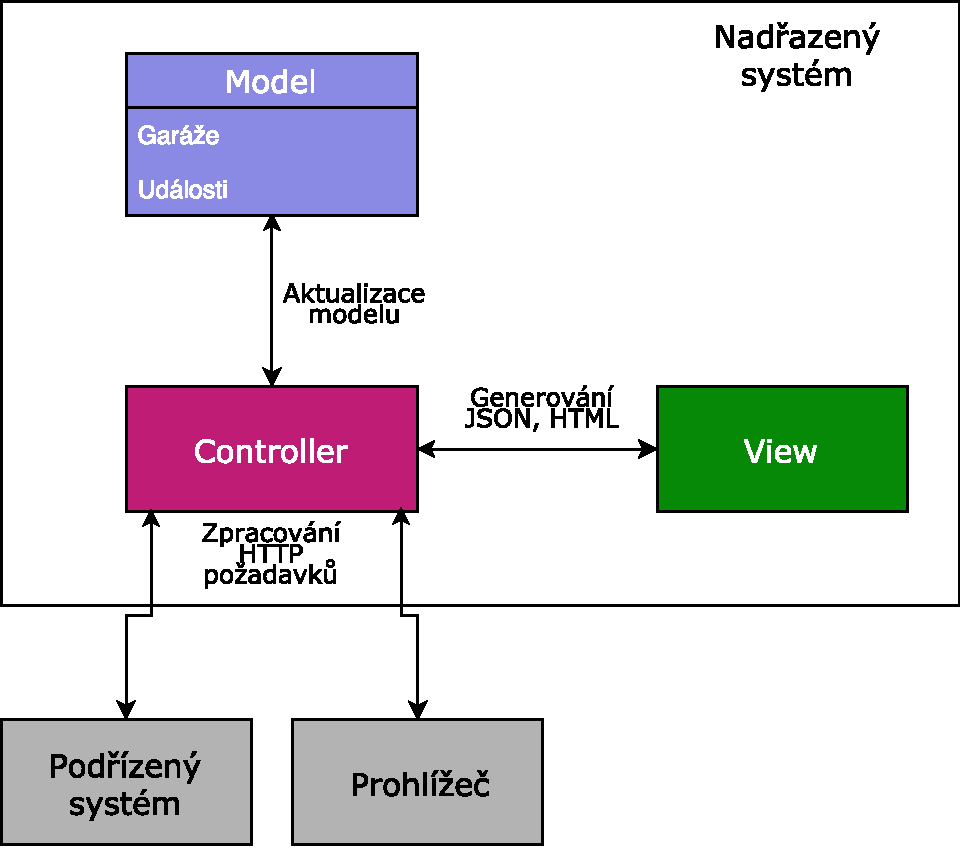
\includegraphics[width=\textwidth]{images/mvc.pdf}
    \caption[Struktura MVC aplikace]{Struktura MVC aplikcace. Uživatel i podřízený systém používají aplikaci pomocí \textit{controlleru}. Ten definuje příslušná URL a zpracovává požadavky na ně -- aktualizuje \textit{model}, případně doručí odpovídající \textit{view}}
    \label{fig:mvc}
\end{figure}

Hlavní motivací pro použití tohoto vzoru je snadná rozšiřitelnost. Pokud by například bylo potřeba aplikaci doplnit o~komunikaci s~podřízenými systémy pomocí MQTT, stačí pouze vytvořit vhodný \textit{controller}. Ten pak může využívat \textit{model} aplikace stejným způsobem jako HTTP \textit{controller}.

Tento návrhový vzor popisuje pouze nadřazený systém spravující garáže. Kromě toho je součástí aplikace ještě autentizace uživatele při přístupu do uživatelského rozhraní. Tuto funkci jsem se rozhodl pojmout jako samostatnou komponentu, popsanou v~sekci \ref{sec:de_auth}.

\section{\textit{Model}}

\textit{Model} představuje jádro nadřazeného systému. Je zde implementována vnitřní reprezentace uchovávaných dat, což jsou především zaznamenané události. Každá událost má také svého původce, tedy garáž (přesněji podřízený systém v~této garáži).

Kromě toho \textit{model} implementuje \textit{business logiku} sytému, tedy například vytváření nových garáží (registraci podřízených systémů) či reakce na příchozích události.

Ostatní části aplikace (\textit{view} a \textit{controller}) používají \textit{model}, bez znalosti jeho vnitřní struktury, pomocí následujících operací:

\begin{itemize}
    \item \textbf{Vytvoření garáže} -- registrace nového podřízeného systému. V~případě vytváření pomocí API (tj. přímo podřízeným systémem) vyžaduje operace zapnutý registrační mód. Pokud je nová garáž vytvářena ve webovém rozhraní, registrační mód není vyžadován.
    \item \textbf{Editace garáže} -- například změna označení.
    \item \textbf{Smazání garáže} -- smazáním garáže dojde k~odstranění zaznamenaných událostí a zneplatnění příslušného API klíče.
    \item \textbf{Zneplatnění API klíče} -- odepření přístupu podřízenému systému bez nutnosti smazání garáže a s~ní spojených událostí.
    \item \textbf{Zapínání/vypínaní registračního módu} -- v~tomto módu je možné vytvářet nové garáže na základě požadavku od podřízeného systému. Bližší informace jsou v~sekci \ref{sec:de_add_garage}.
    \item \textbf{Přístup k~uloženým datům} -- obecně operace typu získání všech garáží nebo všech událostí vázané ke konkrétní garáži.
    \item \textbf{Vytvoření události} -- základní požadavek využívaný podřízenými systémy.
\end{itemize}

Vnitřně pak model na základě těchto operací autentizuje pomocí API klíčů požadavky podřízených systému, validuje zaslaná data a spravuje databázi nadřazeného systému.

\subsection{Garáž -- \texttt{Garage}}

Třída \texttt{Garage} reprezentuje konkrétní podřízený systém a uchovává s~ním spojená data:

\begin{itemize}
    \item \texttt{id} -- identifikace entity v~databázi.
    \item \texttt{tag} -- uživatelem zvolené označení garáže. To slouží pro snadnější orientaci ve webovém rozhraní (uživatel nemusí garáže rozlišovat podle nic neříkajícího \texttt{id}).
    \item \texttt{note} -- poznámka pro další popis garáže.
    \item \texttt{api\_key} -- klíč umožňující přístup k~API systému. Ten je také zaslán zařízení při jeho registraci. Generování a správa klíčů je blíže popsána v~sekci \ref{sec:de_apikeys}.
    \item \texttt{last\_report} -- datum a čas posledního kontrolního hlášeí.
    \item \texttt{next\_report} -- datum a čas dalšího očekávaného hlášení.
    \item \texttt{period} -- perioda kontrolních hlášení.
    \item \texttt{doors} -- stav dveří garáže (otevřeno/zavřeno).
    \item \texttt{state} -- celkový stav garáže (v~pořádku, nehlásí se atd.).
    \item Seznam událostí spojených s~touto garáží.
\end{itemize}

\subsubsection{Vytváření nových garáží}
\label{sec:de_add_garage}

Nové garáže mohou v~systému vznikat dvěma způsoby. První možnost je vytvoření nové garáže přímo v~uživatelském rozhraní. Po vytvoření se zde zobrazí vygenerovaný API klíč, který je potřeba nahrát na příslušný podřízený systém. Způsob nahrávání by závisel na příslušném hardwaru (například sériová linka). Tato možnost je určena především pro podřízené systémy, které by nepodporovaly zaslání registračního požadavku a nevyžaduje zapnutý registrační mód.

Druhá možnost je použít registrační mód. V~tom případě je nová garáž vytvořena na základě registračního požadavku podřízeného systému. Vygenerovaný API klíč je při tom zaslán jako odpověď na požadavek, a není tedy nutné ho ručně nahrávat. Registrační mód je možné aktivovat v~uživatelském rozhraní. Pokud mód není aktivovaný, nadřazený systém odmítne všechny požadavky na registraci zaslané tímto způsobem.

\subsubsection{API klíče}
\label{sec:de_apikeys}

Podřízené systému se při zasílání událostí přes API prokazují klíčem. Ten slouží jednak k~zamezení příjmu událostí od neautorizovaných systému, jednak k~identifikaci původu události (zdrojové garáže) v~rámci nadřazeného systému. Podřízený systém tedy nemusí znát \texttt{id} garáže, ale jen \texttt{api\_key}.

%generovani klice
Vzhledem k~těmto požadavkům nelze použít jeden univerzální, ale je nutné pro každý registrovaný podřízený systém vygenerovat unikátní klíč. Ten je pak spolu s~dalšími záznamy o~garáži uložen v~databázi systému. K~vytváření klíčů jsem se rozhodl použít systém UUID, umožňující generování náhodných klíčů délky 128 bitů, které jsou (pro praktické účely) unikátní \cite{rfc4122}.

Klíče je možné v~uživatelském rozhraní zneplatnit, a tím odepřít přístup zvolenému podřízenému systému. Tuto operaci lze provést dvěma způsoby. V~prvním případě lze smazat z~databáze celý záznam příslušné garáže. Tím dojde k~zneplatnění jejího klíče, ale také k~odstranění zaznamenaných událostí.

Pokud si uživatel přeje data o~událostech uchovat, může pouze vygenerovat nový API klíč. Přepsáním klíče se opět zneplatní přístup podřízeného systému (který má stále starý klíč), ale uchovají se zaznamenaná data. 

Nově vygenerovaný klíč pak uživatel může nahrát na jiný podřízený systém, a tím například nahradit odcizené monitorovací zařízení. V~tomto případě nelze pro nahrání klíče použít registrační mód nadřazeného systému. Ten totiž vždy počítá s~vytvořením nové garáže.

Vygenerované klíče jsou v~databázi uloženy v~čitelné podobě. Klíče by bylo možné před uložením \textit{hashovat}, čímž by při úniku databáze nedošlo k~jejich prozrazení. V~tom případě by byl klíč v~čitelné podobě v~uživatelském rozhraní zobrazen pouze jednou, při vytvoření nové garáže. Dále už by byl uchováván jeho \textit{hash}.

Pro ukládání klíčů v~čitelné podobě jsem se rozhodl především z~důvodů snadného ladění při implementaci nadřazeného a podřízených systémů. Funkci \textit{hashování} klíčů by v~případě potřeby neměl být problém doplnit.

\subsection{Událost -- \texttt{Event}}
\label{sec:de_event}

Třída \texttt{Event} představuje událost zaznamenanou podřízeným systémem. Jak bylo zmíněno v~sekci \ref{sec:de_mvc}, jsou tyto události vázány ke konkrétním garážím, kdy každá událost má jednoznačně určeného původce, a každá garáž libovolné množství událostí.

Nadřazený systém rozlišuje dva základní druhy událostí. Kontrolní (plánované) události slouží ke kontrole funkčnosti podřízených systémů. Tyto události jsou odesílány v~pravidelném intervalu, určeném nadřazeným systémem. Ten v~odpovědi na požadavek s~kontrolní událostí zašle očekávaný čas (počet minut) do dalšího hlášení. Kontrolní událost funguje pouze jako známka života podřízeného systému.

Kromě kontrolních hlášení mohou podřízené systémy vytvářet mimořádné události. Mimořádná událost nastane při překročení mezních hodnot některého z~čidel (tedy detekce kouře, pohybu či otevření/zavření dveří).

Třída \texttt{Event} obsahuje tyto údaje:

\begin{itemize}
    \item \texttt{id} -- identifikace entity v~databázi.
    \item \texttt{timestamp} -- časové razítko.
    \item \texttt{type} -- typ zaznamenané události (kontrolní hlášení, detekce kouře atd.)
    \item Garáž, která je původcem události.
\end{itemize}

\subsubsection{Vyhodnocení události}

notifikace atd..., mozna tuhle sekci nak premenovat.

nakreslit stavovej automat, podle kteryho budou ty prichozi udalosti (a \texttt{check\_report}) menit stav ty garaze. Tj garaz bude ok a prijde ze hori, tak se to zmeni na hori, pak bude check report tak jestli to zas zmeni a tak. Tenhle stavovej automat pak bude implementovanej pomoci tech \texttt{proc\_} metod. plus teda to tlacitko na reset stavu, plus napsat ze votvirani a zavirani dveri je teda zvlast

\section{\textit{Controller}}

Flask API

\subsection{API}

dulezita je idempotence prikazu, tj. bude prikaz na udalost votevreno a na udalost zavreno ale ne toggle, aby se nerozbil stav garaze na serveru.

https://docs.microsoft.com/en-us/azure/architecture/best-practices/api-design

\section{\textit{View}}

\subsection{Uživatelské rozhraní}

\begin{figure}[h!]
    \centering
    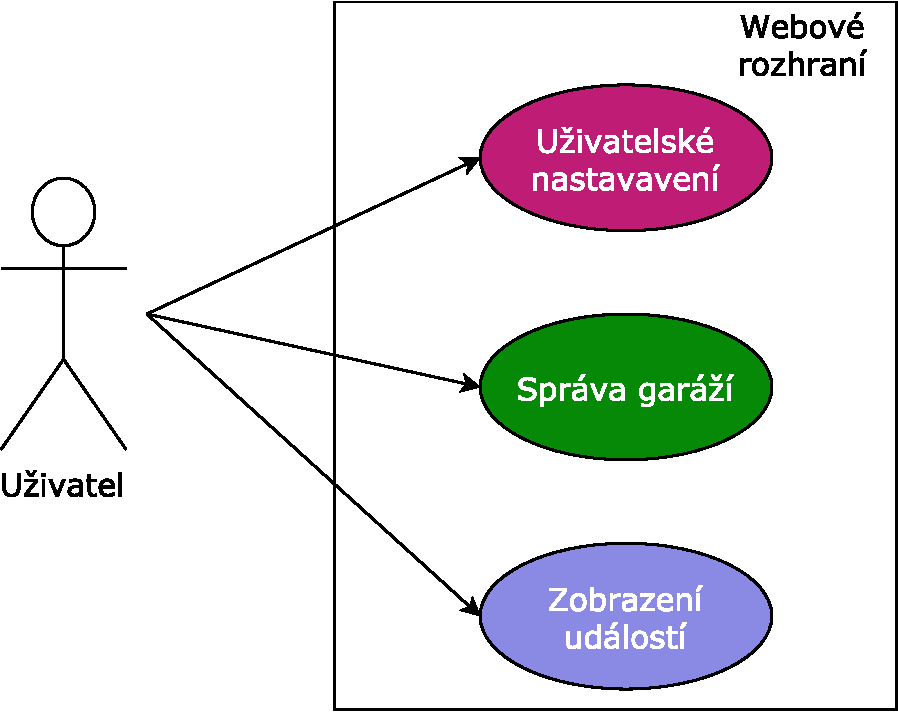
\includegraphics[width=0.9\textwidth]{images/use_case_top.pdf}
    \caption[Vrchní úroveň případů užití webového rozhraní]{Vrchní úroveň případů užití webového rozhraní. Uživatel do aplikace přistupuje buď za účelem změny uživatelského nastavení, správy jednotlivý podřízených systémů, případně kvůli kontrole zaznamenaných událostí}
    \label{fig:use_case_top}
\end{figure}

\begin{figure}[h!]
    \centering
    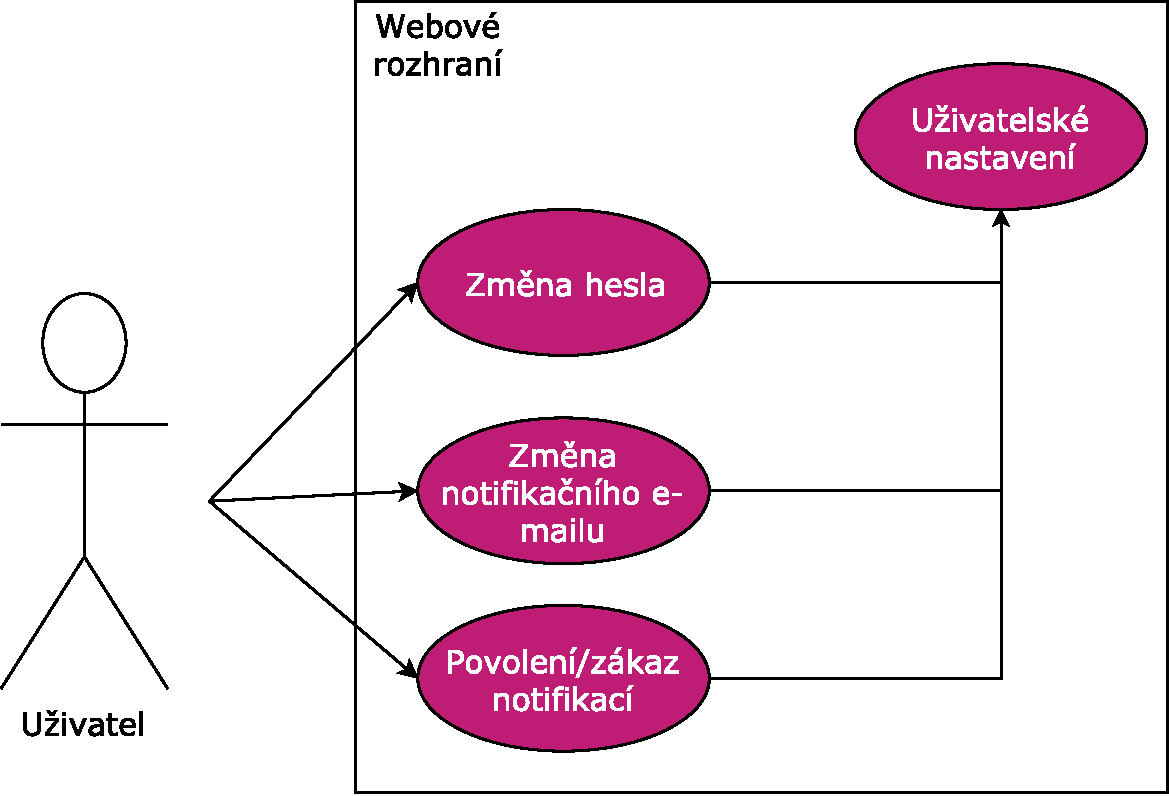
\includegraphics[width=\textwidth]{images/use_case_user.pdf}
    \caption[Případy užití uživatelského nastavení]{Případy užití uživatelského nastavení. Uživatel ve webovém rozhraní provádí změnu hesla, změnu notifikačního e-mailu, případně zákaz/povolení notifikací}
    \label{fig:use_case_user}
\end{figure}

\begin{figure}[h!]
    \centering
    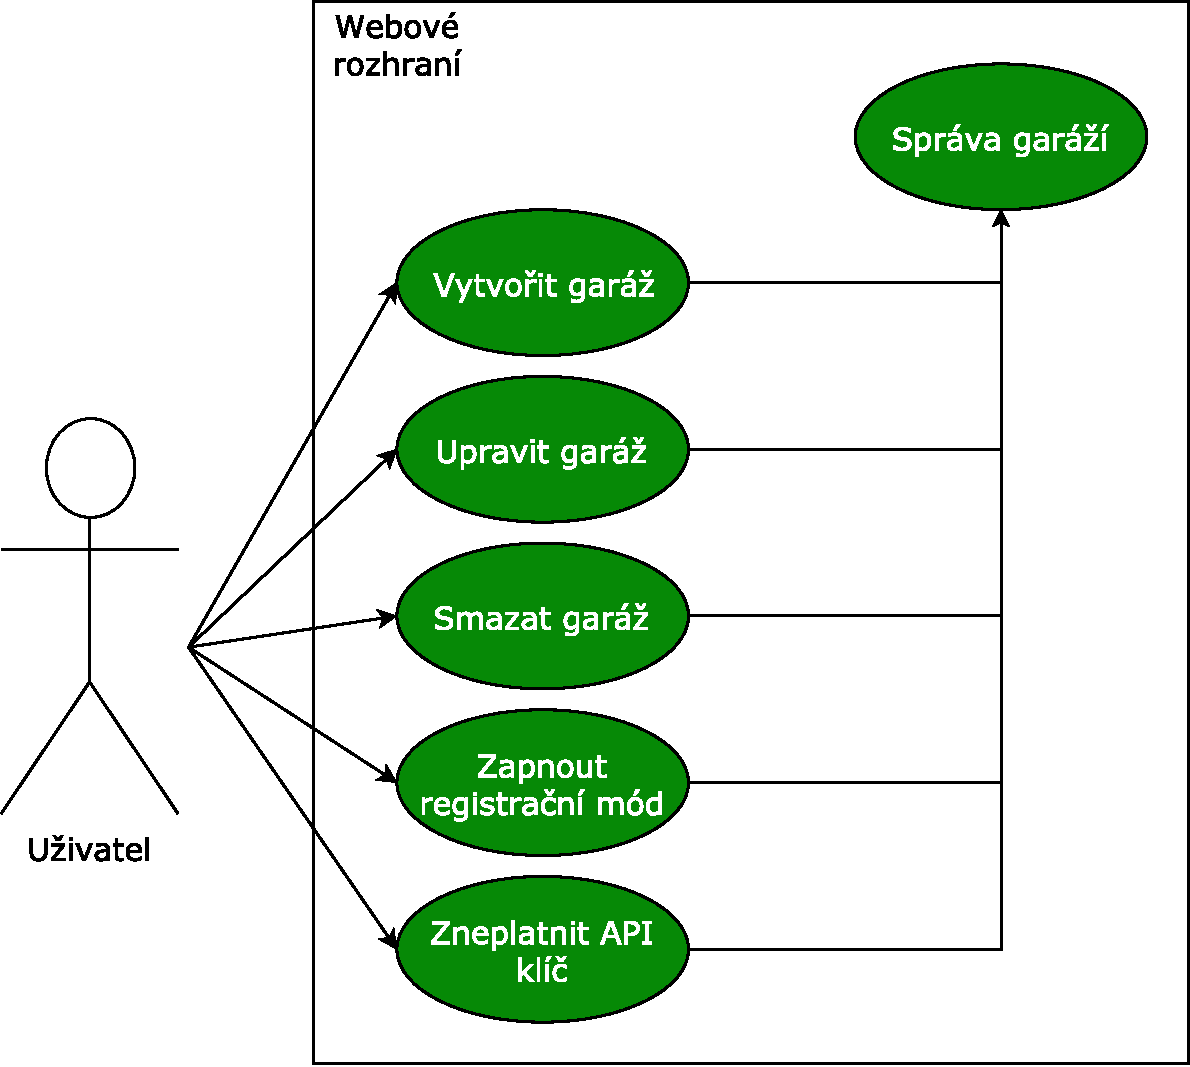
\includegraphics[width=\textwidth]{images/use_case_garage.pdf}
    \caption[Případy užití správy garáží]{Případy užití správy garáží. Zde uživatel zobrazuje stav garáží a jednotlivé garáže spravuje pomocí uvedených operací}
    \label{fig:use_case_garage}
\end{figure}

\begin{figure}[h!]
    \centering
    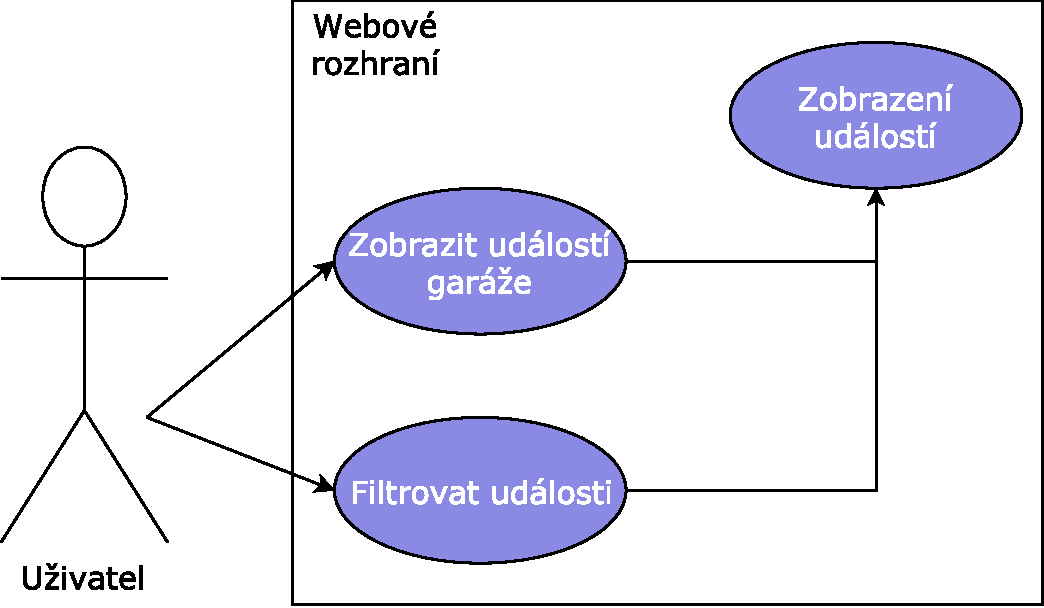
\includegraphics[width=\textwidth]{images/use_case_events.pdf}
    \caption[Případy užití zobrazení událostí]{Případy užití zobrazení událostí. Uživatel zobrazuje událostí spojené s~konkrétní garáží. Událostí filtruje podle jejich typu (viz \ref{sec:de_event})}
    \label{fig:use_case_events}
\end{figure}

\section{Autentizace uživatele}
\label{sec:de_auth}

Do webového rozhraní aplikace je povolen pouze autorizovaný přístup, a je tedy nutné nějakým způsobem ověřit identitu uživatele. Jelikož aplikace nepočítá s~odlišnými stupni přístupu (a tedy každý uživatel s~přístupem do rozhraní má přístup ke všem jeho částem), rozhodl jsem se, že nebudu vytvářet infrastrukturu uživatelských účtů, protože by měla pouze omezené využití.

Přístup do rozhraní tedy nevyžaduje vytvoření účtu a zadávání uživatelského jména, ale pouze heslo. \textit{Hash} tohoto hesla (doplněného solí), vytvořený pomocí algoritmu Bcrypt, je uložen v~souboru s~uživatelským nastavením aplikace.

\textit{Hashování} hesla je zde použito především pro případ, že by uživatel použil stejné heslo jaké používá v~jiných aplikacích či službách. V~případě prozrazení uživatelských dat (například při odcizení systému) tedy útočník nemůže z~otisku zjistit původní použité heslo, tudíž přístup k~těmto uživatelovým účtům není kompromitován.

Stejně tak někdo s~přístupem k~serveru, na kterém nadřazený systém běží, nemá automaticky přístup do webového rozhraní. Nicméně má stále přístup k~celé (nešifrované) databázi a také může heslo libovolně měnit (spočítáním nového otisku), tedy z~praktického hlediska je přístup k~serveru téměř ekvivalentní s~přístupem do webového rozhraní.

\subsection{První přihlášení}

Při prvním startu nadřazeného systému je zvoleno jednoduché implicitní heslo (\textit{password}), kterým se uživatel může přihlásit do webového rozhraní. 

Pokud nadřazený systém detekuje použití tohoto hesla, po přihášení uživatele ihned přesměruje na stránku umožňující změnu hesla a zobrazí příslušné varování.

\section{Uživatelské nastavení}

este teda napsat ze vsechny ty veci spojeny s~uzivatelem nebudou ulozeny v~ty databazi ale jen v~nakym konfiguraku (veci jako heslo a pripadne ten notifikacni mail)
